\section{Implementation}
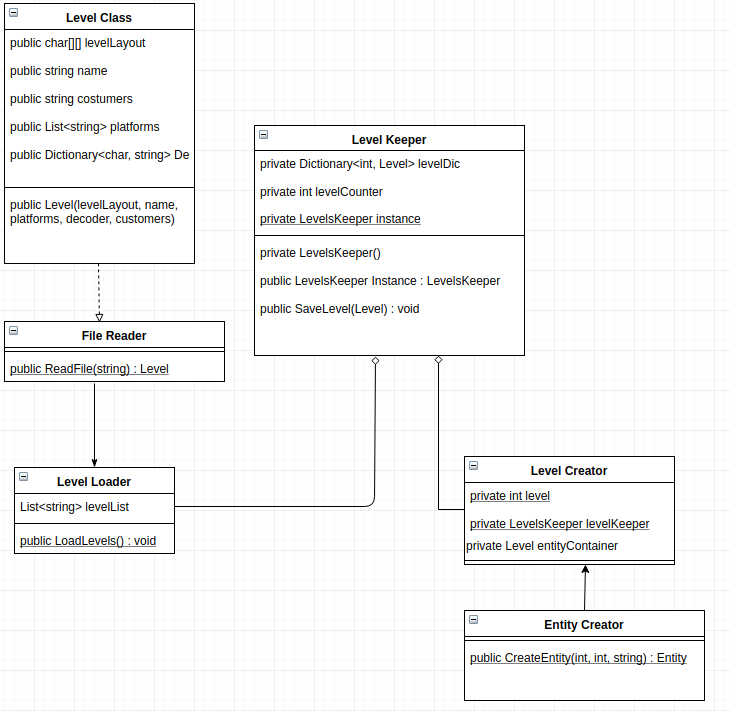
\includegraphics[width=\linewidth]{latex/Images/UML.png}

Som det ses på vores class diagram så er de fleste af vores klasser statiske. Da vi ikke skal bruge flere instanser af for eksempel LevelLoader så vi det mere intuitivt at holde Program og Game fri for objekter som kun skal benyttes en eller få gange, og i stedet bare lade dem kalde statiske metoder i de statiske klasser. Vi vil dog gerne ændre formindske antallet af statiske klasser til inden deadline for eksamen.\\
Undtagelser på det ovenstående er vores Level class som instatierer Level objekter. Da vi ønsker at benytte vores Level objekter som en måde at lagre information om vores levels, har vi valgt kun at implementere en konstruktor til dem og ellers gemme alle informationer i public properties uden setters. Dette garanterer at når Level først er blevet instantieret kan dens informationer ikke overskrives, men informationerne kan til enhver tid læses.\\
En anden undtagelse er LevelsKeeper. LevelsKeeper fungerer som en database for vores levels, og indeholder en dictionary af level numre som keys og Level objekter som values. LevelsKeeper er implementeret som en singleton. Dette er gjort for at arbejde med værdier frem for referencer hvilket bevirker at vi ikke skal bekymre os om hvad der sker hvis der læses og skrives til den samme hukommelse samtidigt. Som det fremgik af vores sequence diagram vil dette ikke kunne lade sig gøre med den nuværende implementation, men skulle det blive nødvendigt at udvide vores model med endnu en klasse som skriver til LevelsKeeper samtidigt med at spillet kører, så kan dette sikkert implementeres. Alternativt ville vi kunne have lavet LevelsKeeper static, men så ville vi skulle være sikre på at der aldrig ville skulle skrives og læses det samme sted samtidigt.\\
At LevelsKeeper er en singleton bevirker at både LevelLoader og LevelCreator skal holde en variabel for LevelsKeeper objektet, som kan kalde sin private metode til at gemme et Level objekt, eller kan benytte sin public property til at returnere et level hvis den er givet et indeks. Metoden er privat, og propertien har ingen setter for at følge princippet om at hver class udfører opgaverne for sit eget ansvar.\\
Vi har lavet collision detection i denne opgave, her har det været nødvendigt at kende forskel på om man er stødt ind i en blok eller en platform. Dette har vi gjort ved at når LevelCreator laver et level returnerer den et array af EntityContainers, som GameRunning da kan render og lave collision detection på. Collision detection foregår først på index 0 i arrayet af EntityContainers som består af alle platformene, det vil sige at hvis der er kollision her ved vi at man har ramt en platform, og vi kan da fortsætte med de nødvendige efterfølgende checks. Derefter checker den næste index, som består af alle blokkene, hvis en af disse rammes slutter spillet. Hvis der ikke er kollision i nogle af de to EntityContainers tjekkes det om Taxien er over toppen af skærmen, hvis dette er tilfældet ved vi at man er fløjet gennem hullet i toppen af skærmen og næste level loades. I starten havde vi overvejet om vi skulle lave to klasser der arvede fra Entity, hvor den ene klasse kan beskrive en blok, og den anden en platform. Hvis vi havde gjort dette kunne vi nøjes med én EntityContainer der består af både bloks og platforme, vi ville da kunne tjekke typen af den Entity der er stødt ind i. Denne implementation ville dog kræve at vi tjekker typen af det objekt der er stødt ind i, dermed have if-statements der tjekker typen, dette ville være et brud på Open/Close princippet \footnote{Kilde: SU18-B4-03-Design\_Patterns, undervisningsmateriale}. 
